\documentclass[12 pt, a4paper]{article}% тип документа, размер шрифта
\usepackage{cmap}	
\usepackage{hyperref}
\hypersetup{
	colorlinks=true,
	linkcolor=blue,
	urlcolor=blue,
}
\usepackage{mathtext}
\usepackage[T2A]{fontenc}%поддержка кириллицы в ЛаТеХ
\usepackage[utf8]{inputenc}%кодировка
\usepackage[english,russian]{babel}
\usepackage{indentfirst}

\usepackage{amsmath,amsfonts,amssymb,amsthm,mathtools} % AMS
\usepackage{amsmath}%удобная вёрстка многострочных формул, масштабирующийся текст в формулах, формулы в рамках и др.
\usepackage{amsfonts}%поддержка ажурного и готического шрифтов — например, для записи символа {\displaystyle \mathbb {R} } \mathbb {R} 
\usepackage{amssymb}%amsfonts + несколько сотен дополнительных математических символов
\frenchspacing%запрет длинного пробела после точки
\usepackage{setspace}%возможность установки межстрочного интервала
\usepackage{indentfirst}%пакет позволяет делать в первом абзаце после заголовка абзацный отступ
\onehalfspacing%установка полуторного интервала по умолчанию
\usepackage{graphicx}%подключение рисунков
\graphicspath{{images/}}%путь ко всем рисункам
\usepackage{caption}
\usepackage{float}%плавающие картинки
\usepackage{tikz} % это для чудо-миллиметровки
\usepackage[export]{adjustbox}
\usepackage{pgfplots}%для построения графиков
\pgfplotsset{compat=newest, y label style={rotate=-90},  width=10 cm}%версия пакета построения графиков, ширина графиков
\usepackage{pgfplotstable}%простое рисование табличек
\usepackage{lastpage}%пакет нумерации страниц
\usepackage{comment}%возможность вставлять большие комменты
\usepackage{float}
%%%%% ПОЛЯ
\setlength\parindent{0pt} 
\usepackage[top = 2 cm, bottom = 2 cm, left = 1.5 cm, right = 2 cm]{geometry}
\setlength\parindent{0pt}
%%%%% КОЛОНТИТУЛЫ
\usepackage[shortlabels]{enumitem}

\usepackage{array,tabularx,tabulary,booktabs} % Дополнительная работа с таблицами
\usepackage{longtable} % Длинные таблицы
\usepackage{multirow} % Слияние строк в таблице
\usepackage{colortbl} % Цветная заливка в таблице
\usepackage[labelsep=period,labelfont=rm,tablename={Таблица},tablewithin=none]{caption}
\usepackage{makecell} 
\usepackage{ctable} % for \specialrule command 

\usepackage{fancybox, fancyhdr}
\pagestyle{fancy} 
\fancyhead[L]{\textit{6 класс}}
\fancyhead[C]{\textit{{ЛМШ "Алые паруса" 2023}}}
\fancyhead[R]{\textit{11 июня}} % ЛЮБАЯ ДОПОЛНИТЕЛЬНАЯ ИНФОРМАЦИЯ
%\fancyfoot[R]{Задание с двух сторон!}
\renewcommand{\footrulewidth}{0.3 mm}

\usepackage{tikzsymbols}
\usepackage{textcomp}
\usepackage{parskip}
\usepackage{graphicx}
\graphicspath{{pictures/}}
\DeclareGraphicsExtensions{.pdf,.png,.jpg}
\usepackage{wrapfig}
%%% Заголовок

%%% Новые команды
\newcommand{\z}[1]{{{\vspace{0.6cm} \large\textbf{{Задача {#1}} \\ }}}}
\newcommand{\task}[1]{{{\vspace{0.6cm} \vspace{-2ex} \textbf{№{#1}}  }}}
\newcommand{\otv}{{\vspace{0.3cm} \textbf{Решение: } \\}}
\newcommand{\uk}{\underline{\textit{Указание.}} }
\newcommand{\opr}{\textit{Определение: }}
\newcommand{\sol}[1]{{{\vspace{0.3cm} \textbf{{Задача {#1}} }\\ }}}
\newcommand{\RomanNumeralCaps}[1]
{\MakeUppercase{\romannumeral #1}}

\usepackage{cancel}
\usepackage{epigraph} 
\setlength\parindent{0pt}
\setlength\parskip{1ex plus 2pt minus 1pt}
\newcommand\X{\par\noindent---~}
\usepackage{ upgreek }
\begin{document} % конец преамбулы, начало документа
	\newpage
	\begin{flushright}
		\textit{<<Все мы - связанный граф, но сможем ли мы когда-нибудь стать полным графом...>>}
	\end{flushright}
	\begin{figure}[t]
		\begin{minipage}[h]{0.33\linewidth}
			
\includegraphics[width=0.33\linewidth, left]{logo.jpg}
		\end{minipage}
		%%	\hfill
		\begin{minipage}[h]{0.33\linewidth}
			\centering
			\large{\textbf{ГРАФЫ}}\\
		\end{minipage}
		\begin{minipage}[h]{0.33\linewidth}
			
\includegraphics[width=0.33\linewidth, right]{logo.jpg}
		\end{minipage}
		\label{ris:image1}
	\end{figure}
	
	\begin{comment}
		\begin{figure}[b]
			\begin{minipage}[h]{0.33\linewidth}
				
\includegraphics[width=0.33\linewidth, left]{logo.jpg}
			\end{minipage}
			%%\hfill
			\begin{minipage}[h]{0.33\linewidth}
				\centering
				\large{\textbf{Удачи \Winkey}}
			\end{minipage}
			\begin{minipage}[h]{0.33\linewidth}
				
\includegraphics[width=0.33\linewidth, right]{logo.jpg}
			\end{minipage}
			\label{ris:image1}
		\end{figure}
		
		\begin{tabular}{lcr}
			
\includegraphics[width=0.2\linewidth]{logo.jpg} &
			\vspace{-2ex}
			\large\textbf{Вступительная работа} &
			
\includegraphics[width=0.2\linewidth]{logo.jpg}
		\end{tabular}
	\end{comment}
	
	\large
	\raggedright
	\textbf{\textit{Граф}} - это конечное множество точек на плоскости, некоторые
	пары которых соединены линиями. Эти точки называются вершинами, а линии -
	ребрами графа.\\
	\textbf{\textit{Степень вершины}} - это количество ребер выходящих из вершины графа.
	
	\task{1} В графе с \cancel{5} n вершинами любые две вершины соединены ребром. Сколько
	всего рёбер в этом графе?\\
	\task{2а} Можно ли расставить цифры от 1 до 9 по кругу так, чтобы сумма никаких двух
	соседних чисел не делилась ни на 3, ни на 5, ни на 7?\\
	\vspace{-1ex}
	\task{2б}Можно ли записать цифры от 0 до 9 в строку так, чтобы число, составленное
	из любых двух подряд идущих цифр, делилось на 7 или на 13?\\
	
	\task{3}Каждые 5 минут случайные два призрака отправляют детей возрождаться.
	Оказалось, что каждый отправил детей возрождаться ровно три раза. Могло ли так оказаться, что к тому моменту прошло ровно 895 минут?
	
	\task{4} Как связаны сумма степеней вершин и кол-во рёбер?\\
	
	\task{5a} \textbf{Лемма о рукопожатиях.} Докажите, что чётно число людей, которые в своей
	жизни сделали нечётное число рукопожатиий.\\
	
	\task{5б} Верно ли, что число вершин нечётной степени любого графа чётно?\\
	
	\task{6} В некой компании из шести человек любые двое либо знакомы друг с другом, либо не
	знакомы. Докажите, что среди этих шести человек найдутся трое попарно знакомых или трое попарно незнакомых.\\
	
	\task{7} Сколько ребер куба (максимум) можно перекусить посередине, чтобы
	он не распался на части?\\
	
	\textit{\textbf{Эйлеровым графом}} называется граф, в котором есть \textit{эйлеров цикл}.\\
	\textbf{\textit{Эйлеров цикл}} - это путь, проходящий по всем рёбрам графа и притом только по одному разу\\
	
	\newpage
	
	\task{8а} Через город Кенигсберг протекает река, в русле которой расположены два
	острова. С большего острова ведет по два моста на каждый из
	берегов и один мост на меньший остров. Кроме этого
	моста с меньшего острова ведет по одному мосту на
	каждый из берегов. Некто хочет совершить прогулку по
	городу, пройдя по каждому мосту ровно один раз. Удастся ли ему это?\\
	\task{8б} Можно ли нарисовать изображенные на рисунках граф не отрывая карандаш от бумаги и проводя каждое ребро ровно один раз?\\
	\begin{center}
		\begin{figure}[h]
			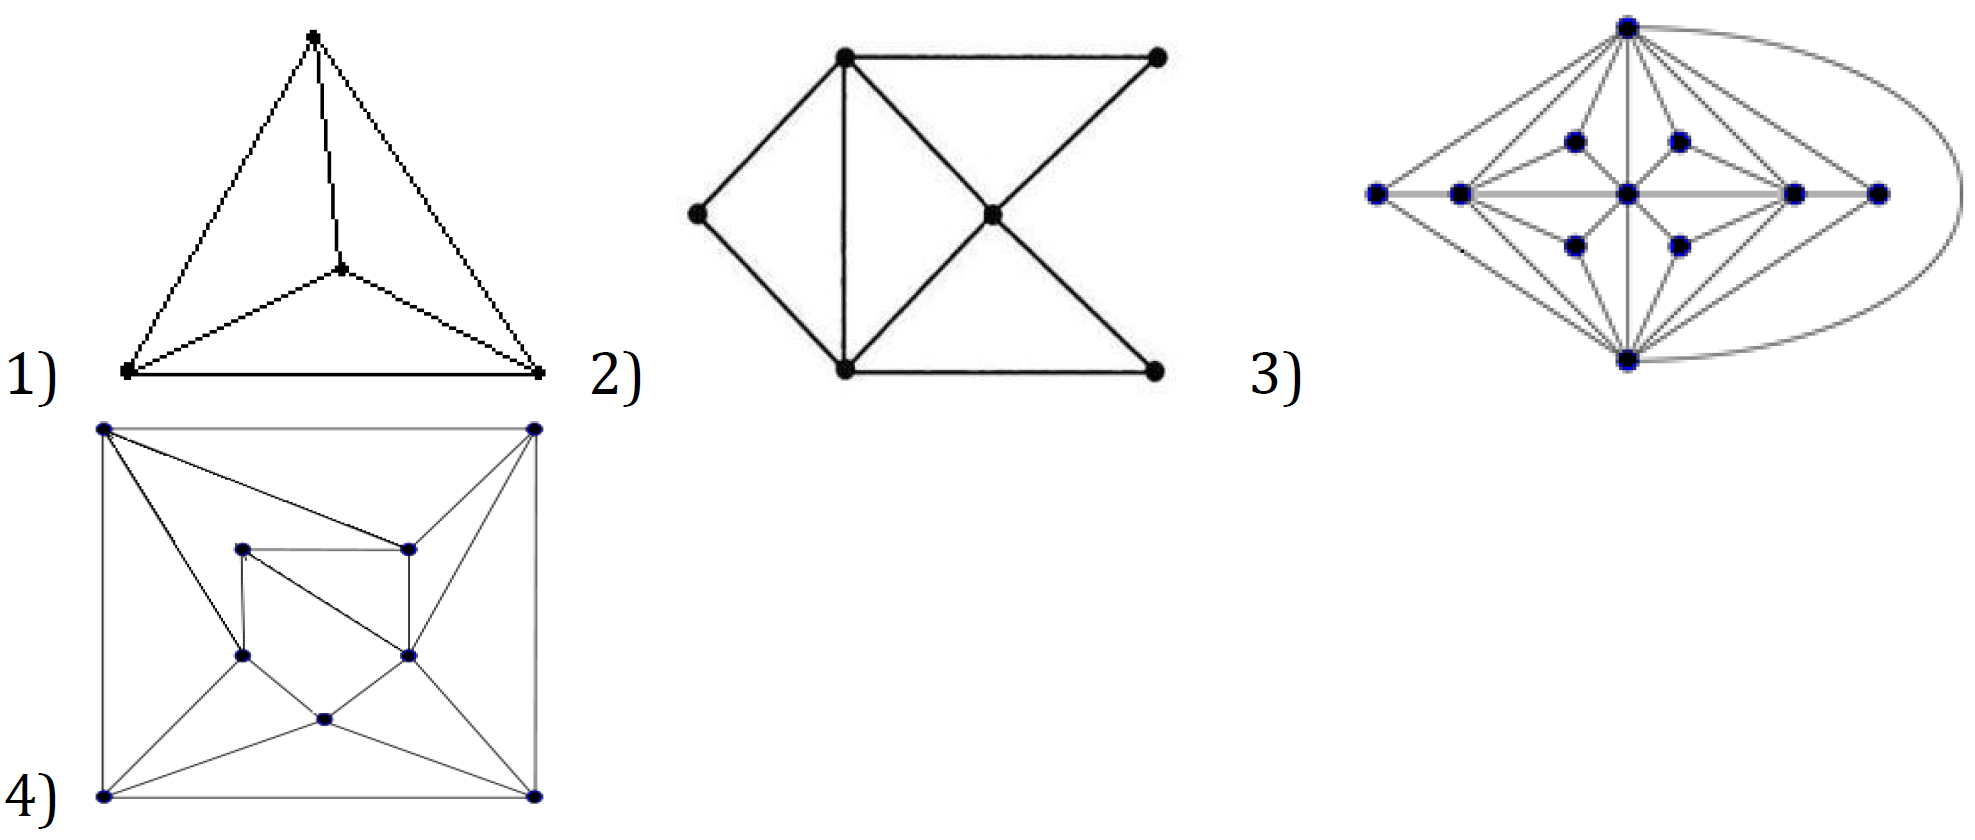
\includegraphics[width=\linewidth]{pic.png}
		\end{figure}
	\end{center}
	\vspace{-6ex}
	\task{8в} Какое условие для графа должно выполняться, чтобы он был эйлеровым.\\
	\task{9а} \textbf{В следующих задачах нужно восстановить исходный граф.} Вначале был граф с пятью вершинами. Для каждой из пяти вершин нарисовали,
	какой граф останется после удаления этой вершины вместе с исходящими из неё рёбрами. Вы видите
	справа пять получившихся графов, каждый в отдельной рамке.\\
	\begin{center}
		\begin{figure}[h]
			\centering
			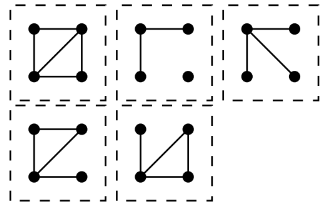
\includegraphics[width=0.33\linewidth]{pic2.png}
		\end{figure}
	\end{center}
	\vspace{-6ex}
	\task{9б} В графе известны степени всех вершин: 6, 5, 3, 3, 2, 2, 1. \\
	\task{9в} В графе известны степени всех вершин: 5, 5, 4, 4, 4, 1, 1. \\
\end{document} 